
\section{Refraction of Light}

\makelabheader %(Space for student name, etc., defined in master.tex)

\bigskip
\textbf{Objective}

To investigate the path traveled by light through a plate of plexiglass
(a transparent solid material).

\bigskip
\textbf{Apparatus} 

\begin{itemize}
\item light fence 
\item plexiglass block 
\item white paper, pins, and wood board 
\item protractor
\end{itemize}

\textbf{Introduction}

The speed of light depends on the medium in which it travels. In passing
from one medium, at least some light energy is reflected. If the second
medium is transparent, most of the light will pass into and through
it. If the beam is not perpendicular to the boundary between the two
media, it will bend as it enters, an effect known as refraction. The
direction a single ray of light travels when refracted is given by
Snell's law:

\begin{displaymath} \frac{sin~i}{sin~r} = \frac{v_1}{v_2} = \frac{n_2}{n_1} \end{displaymath}

where

\begin{quote}
i = incident angle

r = refracted angle

v\( _{1} \) = light speed in medium 1

v\( _{2} \) = light speed in medium 2

n\( _{1} \) = index of refraction of medium 1 

n\( _{2} \) = index of refraction of medium 2
\end{quote}
\textbf{Note}: All angles are measured from the normal to the boundary
at the point the ray enters (or leaves) the medium. The index of refraction is
the ratio of light's speed in a vacuum, $c$, to its speed in the medium,
$v$: $n = c / v$. It is worth remembering that $n_{air} \approx 1.00$.

%\vspace{0.3cm}
{\centering 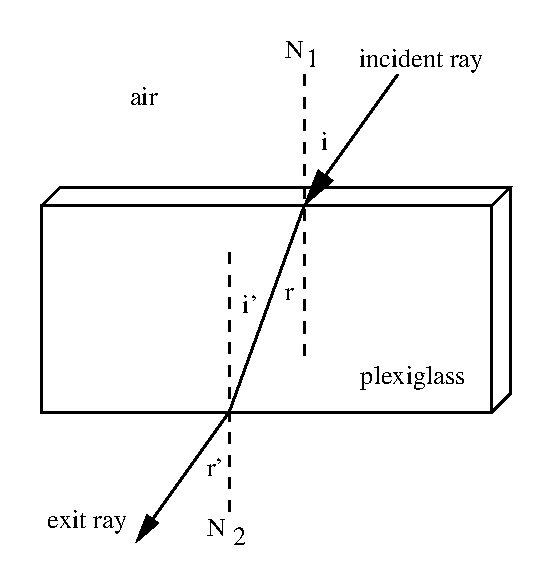
\includegraphics[width=0.35\textwidth]{refraction_of_light/refraction_of_light_fig_1.eps} \par}
%\vspace{0.3cm}

%\vspace{15mm}

\pagebreak[2]
\textbf{Activity} 

\begin{enumerate}[labparts]
\item Put a plexiglass plate at the center of a piece of paper. Outline
its position. Identify a normal, $N_1$, perpendicular to an edge of
the plate.
\item Arrange the light source apparatus so that the parallel rays of light
cross the paper and are incident at a $30^\circ$-$35^\circ$ angle
to the normal. Trace one of these rays.
\item Sight the corresponding ray as it emerges from the other side of the
plexiglass. Trace this ray.
\item Remove the plexiglass and connect the points where the light ray entered 
and left the plexiglass with a straight line. This represents the path of the 
light ray as it passes through the plexiglass.
\item Construct the normal, $N_2$, and measure and record $i$, $r$, $i'$, and $r'$. 
\answerspace{20mm}

\item Repeat the above procedure for two more incident angles between
$40^\circ$ and $60^\circ$. \vspace{30mm}
\item Plot a graph of $sin~i$ (on the vertical axis) as a function of $sin~r$ 
(on the horizontal axis) including the point (0,0) which corresponds to a 
light ray incident perpendicular to the plexiglass. Include a linear trendline 
and don't forget to include a title and axis labels.
\item Use the LINEST function in $Excel$ (see \textbf{Appendix \ref{excel}}) to 
determine the slope of the graph ($n_{plexiglass}$) and its uncertainty.
\vspace{25mm}

\item Does $i = i'$? Explain.\answerspace{20mm}

\item Does $r = r'$? Explain.\answerspace{20mm}

\item Are the incident and exit rays parallel? Explain.\answerspace{20mm}

\item What is the speed of light in the plexiglass?\answerspace{25mm}

\item Under what conditions would a refraction angle be greater than an
incident angle?\answerspace{25mm}
\item Collect the results from the other lab groups and determine an average 
and standard deviation for the index of refraction of the plexiglass.
\end{enumerate}

